\section{Path planning}
\label{sec:path}

\subsection{Augmented graph}
\label{sec:augraph}
To enhance the basic path planning capabilities provided by the Rescue Simulator's sample agent, we create an augmented neighborhood graph that conveys more information about distance among areas. The augmented graph helps guiding agent navigation and Police Force clearing procedures.

In the following discussion, we refer to area as a building or a road, according to the naming in Rescue Simulator's source code. Besides, two areas are considered neighbors if they are adjacent and an agent can move between them in the absence of blockades.

In the sample search graph (available in the Rescue Simulator package), areas are the nodes and an arcs connect neighbor areas. In the augmented graph, a node exists at each door or passage between areas. These nodes are located in the midpoint of the door or passage. Also, an additional node is located at the centroid of each area. Arcs connect all nodes in the same area. 

The augmented graph allows easier and precise computation for its arc weights. The weights are approximated by the euclidean distance between nodes. Weights are more difficult to calculate in the sample search graph as the nodes have no information about position. If the area centroid is considered as their location and weight is given by euclidean distance, large errors could occur as the euclidean distance between centroids may diverge greatly from the distance an agent must actually traverse. Besides, the augmented graph allows more detailed blockade handling: if the path between two adjacent nodes is blocked, we mark only the edge that connects them as impassable. Other edges inside the same area might still be traversable. In the sample search graph, the edges are not associated with positional information, making it difficult to represent detailed blockade information.

%Algorithm \ref{alg:augbuild} shows how the augmented search graph is constructed.
%
%\begin{algorithm}[ht]
%\begin{algorithmic}
%\FORALL{$a \in MapAreas$} 
%\FORALL{$n \in neighbors(a)$} 
%\STATE Insert node at midpoint of $a$-$n$ door/passage
%\ENDFOR
%\STATE Insert node at centroid of $a$
%\ENDFOR
%\end{algorithmic}
%\caption{Augmented graph construction}
%\label{alg:augbuild}
%\end{algorithm}

Figure \ref{fig:graphs} shows the differences on sample and augmented graphs. Nodes in the sample search graph are drawn in area centroid for purposes of illustration, as they do not convey positional information. The graph is augmented with the squared orange nodes.

\begin{figure}[ht]
  \centering
  \subfigure[]{
    {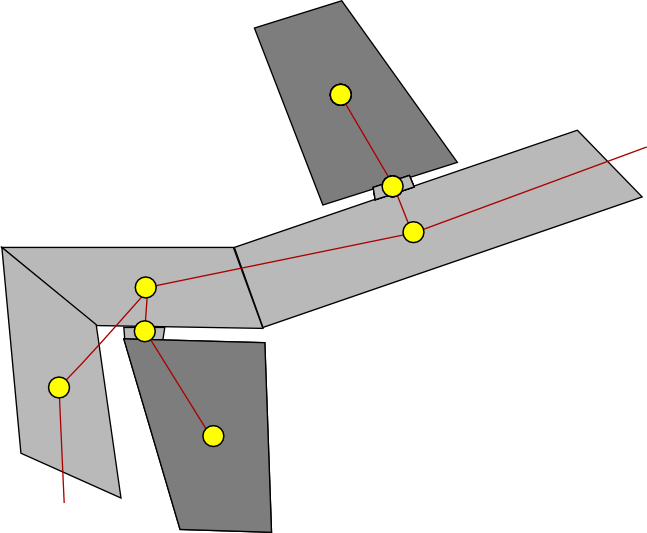
\includegraphics[width=5.2cm]{img/graph-sample.png}}
    \label{fig:sample}
  }
  \subfigure[]{
    {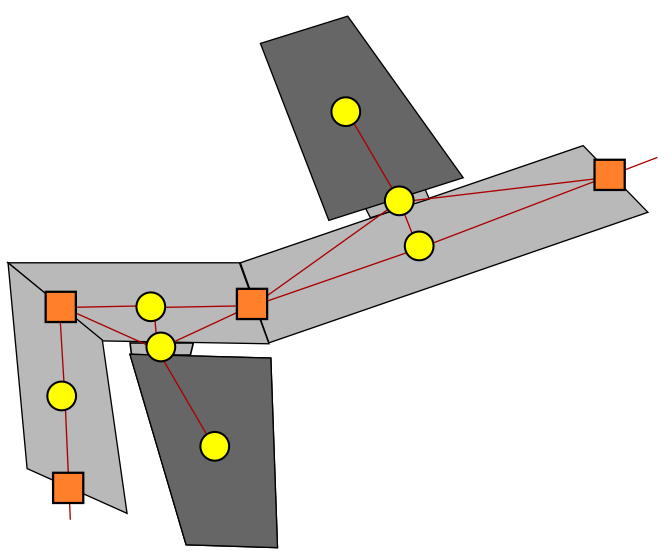
\includegraphics[width=5.2cm]{img/graph-aug.png}}
    \label{fig:aug}
  }%
  \caption{Sample \subref{fig:sample} and augmented \subref{fig:aug} search graphs representing a hypothetical region. Roads are in light gray whereas buildings are in dark gray.}
  \label{fig:graphs}
\end{figure}

Each agent has an instance of the augmented graph. During path planning, an extra node is added at the agent's position. This node is connected to all nodes in the same area, with arc weights assigned via euclidean distance. Path planning proceeds by executing Dijkstra's algorithm with origin as the agent's node and destination as the node at the centroid of the destination area. 

As a measure for robustness, the search falls back to Breadth First Search (BFS) over the sample search graph if the augmented graph cannot be instantiated. 

\subsection{Static and dynamic path planning}
\label{sec:static-dynamic}

Path planning is divided in static and dynamic path planning. Static path planning occurs at the pre-processing stage, where we calculate the shortest path between all pairs of map nodes. %This is done by repeated application of Dijkstra's algorithm. 
Static path planning generates a table with origin-destination pairs and the route between them. During simulation, agents perform a lookup on this table and save processing time to know the shortest path between two nodes. Static path planning works either with BFS over the sample search graph or Dijkstra over the augmented graph.

Dynamic path planning occurs when a blockade is detected in a road. When this happens, the shortest path between the agent's origin and destination is recalculated. With BFS over the sample search graph, the road is marked as blocked whereas with Dijkstra over the augmented graph, the edges that intersect the blockade are marked as blocked. 
The new route is updated in the agent's origin-destinations table and a message is sent to other agents to warn them about the blockade. Upon receipt of this kind of message, agents mark the routes containing the blocked road or edges as invalid on their origin-destination table. When the blockade is cleared by police forces, a new message is sent so that the agents can agents mark the routes containing the blocked road or edges as valid again.
